Aurinkosähköjärjestelmät koostuvat aurinkopaneeleista, aurinkoinverttereistä sekä mahdollisista energiavarastoista. Riippuen järjestelmästä, aurinkopaneeliketjuun tai yk-sittäisiin paneeleihin voidaan kytkeä myös DC/DC-muunnin. Tästä saadaan lisähyötyjä varjostustilanteissa tai epätasaisessa auringonpaisteessa.  Kuvassa 1 näkyy aurin-kosähköjärjestelmän lohkokaavio, joka esittää verkkokytketyn järjestelmän komponentteja.

Järjestelmä tuottaa energiaa vain tiettyyn aikaan päivästä, ja sen tuottoteho voi vaihdella hyvin nopeasti säätilasta riippuen. Kotitaloudessa ylimitoitetut järjestelmät, joissa ei ole hyödynnetty kommunikaatiorajapintoja, syöttävät huipputehoaikana sähköä verkkoon päin. Kommunikaatiorajapintoja hyödyntämällä kotitaloudet voisivat hyödyntää tämän energian itse, liittämällä aurinkosähköjärjestelmän esimerkiksi kodin automaatioon.

Järjestelmän koko, mahdolliset staattiset varjostuskohdat sekä tulevaisuuden laajenta-mistarpeet vaikuttavat järjestelmän suunnitteluun. Invertterin valinta vaikuttaa laite- ja asennuskustannuksiin sekä järjestelmän päivittäiseen energiantuotantoon, mutta myös järjestelmän turvallisuuteen ja suojalaitteiden tarpeeseen. Inverttereiden eri vaihtoehtoja käsitellään myöhemmin omassa kappaleessaan.

Osa kaupallisista järjestelmistä ylittää 1MW tehon. Tällaisille järjestelmille Fingrid asettaa rajoituksia kommunikaation reaaliaikaisuuden osalta; verkonhaltijan on lähetettävä jär-jestelmien mittaustietoja enintään 60 sekunnin päivityssyklillä. Tällöin verkonhaltijan vas-tuulla on toimittaa järjestelmään mittarit täyttääkseen Fingridin vaatimukset reaaliaikaisuudesta.

\section{Aurinkopaneelit}
  Aurinkopaneeleiden toiminta perustuu valosähköiseen ilmiöön. Ne koostuvat suuresta määrästä sarjaan kytkettyjä aurinkokennoja, joista jokainen tuottaa tyypillisesti täydessä auringonpaisteessa hieman alle 5 W tehon noin 0,5 V jännitteellä.

  Aluksi, kun aurinkosähköjärjestelmät olivat pääosin verkosta irti kytkettyjä järjestelmiä, paneelit koostuivat 36 kennosta, koska tuon ajan akut olivat pääosin 12 V lyijyakkuja, joiden latausjännite vaihtelee 14–16 V välillä. Nykyään, kun aurinkosähköjärjestelmät ovat suurimmalta osin verkkoon kytkettyjä, aurinkopaneelien kennojen lukumäärä voi olla huomattavasti suurempi kuin ennen, riippuen järjestelmässä käytettävien invertte-reiden sisääntulojännitteestä.

  Kennot ryhmitellään usein moduuleiksi, joiden kanssa rinnan kytketään ohitusdiodit. Jos kennot varjostuvat, ohitusdiodi ohittaa kyseisen moduulin, jossa varjostuneet kennot si-jaitsevat, jolloin se ei aiheuta häviöitä muualla rajoittamalla muiden moduulien tai panee-leiden virtaa. Usein aurinkopaneelit ketjutetaan tarvittavan jännitteen saamiseksi, jolloin ohitusdiodien apu varjostustilanteissa on erittäin tärkeää, sillä muuten varjostuskohta ra-joittaisi koko paneeliketjun virtaa.

  Aurinkokennojen ja -paneelien toimintakäyrinä käytetään usein virta-jännite -käyrää ja siitä johdettua teho-jännite (engl. P-V) -käyrää. Kuten kuvasta 2 nähdään, P-V-käyrän huippukohdan sijainti vaihtelee valaisutehon mukaan. Tätä käyrän huippukohtaa kutsutaan huipputehopisteeksi (engl. maximum power point, MPP). Se näyttää jännitteen, jolla saavutetaan kennon tai paneelin huipputeho kullakin valaisuteholla.
  \begin{figure}
    \centering
    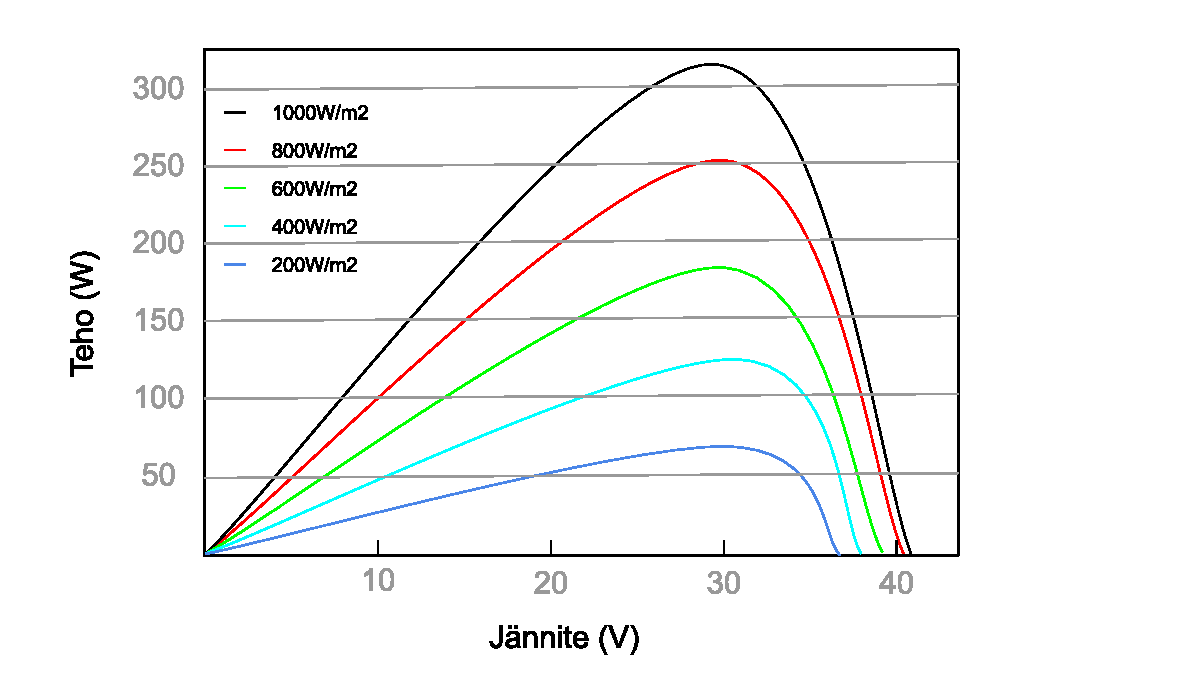
\includegraphics[width=0.5\textwidth]{figures/pvcurve}
    \caption{JA Solarin erään aurinkopaneelin P-V-käyrä eri valaisutehoilla}
  \end{figure}
  Piirillä, jossa on sarjaan kytkettyjä aurinkopaneeleita, on jokaisella paneelilla oma paikal-linen huipputehopisteensä (engl. MPP - Maximum Power Point), mutta myös koko piiril-lä on yhteinen globaali huipputehopiste. Globaali huipputehopiste muuttuu varjostusten ja pilvisyyden mukaan koko järjestelmän tasolla ja sitä tarkkailemalla saadaan selville, millä jännitteellä koko järjestelmästä saadaan suurin teho.

\section{Invertterit}
  Invertteri eli vaihtosuuntaaja on laite, joka muuttaa tasasähköä vaihtosähköksi. Invertte-rin sisääntulojännite vaihtelee käyttötarkoituksen mukaan: kaupalliseen käyttöön tai suu-rempiin järjestelmiin tarkoitetut laitteet toimivat korkealla, jopa 1500V jännitteellä, koska niissä on pidemmät johdotusmatkat ja suurempi määrä paneeleita kytkettynä sarjaan. Kuluttajakäytössä taas voidaan käyttää selvästi pienemmän tason jännitteitä johdotusten ollessa huomattavasti lyhyempiä ja paneeleiden määrän ollessa pienempi.

  Korkeampi jännitetaso keventää huomattavasti tarvittavaa johdotusta, kun virta voidaan pitää pienenä ja siten johtojen läpimitta pienenä. Myös häviöt pienenevät huomattavasti, koska johdoissa syntyvät häviöt kasvavat Ohmin lain
  \begin{equation}
    \textrm{P} = RI^2
  \end{equation}
  mukaan virran suhteen neliöllisenä.

  Invertteri, jolla on valmiudet huipputehopisteen seurantaan (engl. MPP Tracking, MPPT), etsii siihen kytketyn aurinkopaneeliryhmän huipputehopistettä aktiivisesti. Pis-teen etsimiseen käytetään monia eri tekniikoita, mutta tämän työn kannalta niiden läpi-käynti ei ole relevanttia. Jos käytetty tekniikka on liian herkkä löytämään huipputehopis-teitä, se voi valita paikallisen pisteen globaalin sijaan ja aiheuttaa huomattavia tehohäviöitä väärän pisteen valinnalla.

  Aurinkopaneeliryhmän tehoa voidaan muuttaa kuormavastusta säätämällä. Huipputehopisteelle löytyy aina sitä vastaava ominaisvastus kaavan 2
  \begin{equation}
    R_{CH} = \frac{V_{MPP}}{I_{MPP}}
  \end{equation}

  mukaisesti, ja invertteri säätää kuormavastuksen ominaisvastuksen mukaiseen arvoon, löydettyään järjestelmän huipputehopisteen mukaiset arvot kaavaan.

  Invertterit voidaan jakaa pääosin kolmeen eri tyyppiin järjestelmien topologioiden mu-kaan: keskusinverttereihin, mikroinverttereihin sekä ketjuinverttereihin. Keskusinvertterit ovat kaupallisissa kohteissa käytettäviä, suuritehoisia inverttereitä, kun taas mikroinvert-terit ovat pääosin kuluttajakäyttöön suunnattuja laitteita. Ketjuinvertterit sijoittuvat näiden väliin ja laajan tehoskaalan vuoksi niitä voidaan käyttää molempien tyyppisissä kohteissa.

\subsection{Keskusinvertteri}
  Keskusinvertterin teho on usein hyvin suuri, yli 50 kW:sta jopa muutamaan megawattiin. Niitä käytetään suurissa aurinkovoimaloissa, joissa ei usein tarvitse miettiä rakennel-mien tai puiden aiheuttamia varjostuksia. Tällöin asennuskustannukset pienenevät, sillä suuriin järjestelmiin riittää yksi invertteri.

  Keskusinvertterin huonoja puolia ovat järjestelmän riippuvuus yksittäisestä invertteristä sekä vain muutama huipputehopiste koko järjestelmälle. Tällöin järjestelmässä tulee suuret tehohäviöt, jos esimerkiksi pilvi kulkee osittain paneelikentän yli ja huipputehopis-te määräytyy koko järjestelmälle, jolloin täysin auringossa olevien paneelien teho laskee huomattavasti. Käyttökohteiden ja suunnittelun takia tämä ei toisaalta vaikuta merkittä-västi järjestelmän tuottoon.

\subsection{Mikroinvertteri}
  Mikroinvertteri on pienitehoinen vaihtosuuntaaja, joka on joko integroitu aurinkopaneelin yhteyteen tai asennettu sen välittömään läheisyyteen. Tämä tarkoittaa, että jokaiselta paneelilta voidaan säätää sen tehoa huipputehopisteen mukaiseksi. Tällöin saadaan epätasaisissa varjostustilanteissa paras mahdollinen teho, kun jokaisesta paneelista voi-daan maksimoida teho. Tämä johtuu siitä, että yhden paneelin varjostuminen ei vaikuta muiden paneelien tuottoon, koska paneelit eivät ole kytketty sarjaan.

  Mikroinverttereiltä saadaan hyvin paljon tietoa, koska inverttereiden määrä järjestel-mässä on suuri. Tällöin saadaan reaaliaikaisesti kuva järjestelmän toimivuudesta, ja pie-netkin virhetilat voidaan korjata niiden ilmentyessä. Toisaalta inverttereiden määrä ai-heuttaa haasteita tiedon koostamisessa ja tiedonsiirrossa, koska tieto ei ole välttämättä keskitetysti yhdessä paikassa sellaisenaan, vaan voi vaatia ylimääräisiä komponentteja tiedon keräämiseen.

  Kuluttajapuolen ratkaisuissa tiedonhallinta on usein toteutettu verkkokäyttöliittymällä, jol-loin jokainen invertteri on liitetty erilliseen laitteeseen, joka lähettää tiedot valmistajan omaan järjestelmään tiedon koontia varten. Tästä esimerkkinä Enphasen Envoy ja En-vertechin EnverBridge, jotka kommunikoivat valmistajan mikroinverttereiden kanssa PLC-väylän kautta. Sen jälkeen laite lähettää tiedot verkkoportaaliin, josta käyttäjä voi seurata paneelien tuotantoa ja järjestelmän toimivuutta.

\subsection{Ketjuinvertteri}
  Ketjuinvertteriin kytketään nimensä mukaisesti sarjaan kytketyistä paneeleista muodos-tettuja ketjuja. Siinä on usein monta huipputehopisteen seurannan kytkentää, jolloin saadaan seurattua useita huipputehopisteitä invertteriä kohden. Invertterien teho vaihte-lee muutamasta kilowatista jopa satoihin kilowatteihin, jolloin sitä voidaan käyttää hyvin erikokoisissa järjestelmissä.

  Teholuokaltaan pienet ketjuinvertterit on suunniteltu käyttäjäystävällisyyshuomioiden, ja esimerkiksi SMA:n ja Huawein invertterit sisältävät integraation valmistajien taustajärjes-telmiin. SMA on toteuttanut tämän integraation valmiina, kun taas osa Huawein invertte-reistä vaatii sovittimen Ethernet-portin, WLANin tai matkapuhelinverkon käyttämiseen datasiirrossa.

  SMAn invertterit käyttävät lisäksi SunSpec Alliancen Modbus-standardia, joka toimii Et-hernet-portin välityksellä. Muut standardia hyödyntävät valmistajat voivat kommunikoi-da suoraan SMAn inverttereiden kanssa standardoinnin takia. Huawei käyttää myös Modbus-protokollaa, mutta se ei ole SunSpec Alliancen standardoima. Tämä tarkoittaa, että Huawein kanssa kommunikoitaessa sille on kehitettävä oma rajapinta datan luke-miseksi.

  Modbusin hyödyntäminen mahdollistaa muiden valmistajien tuotteiden kommunikaation inverttereiden kanssa. Yhteinen standardi helpottaa suurissa järjestelmissä eri valmista-jien tuotteiden yhteensopivuuden kanssa, mutta ylipäätään Modbusin käyttö antaa mahdollisuuden kolmannen osapuolen tuotteiden liittämiseen.

\section{Järjestelmien tuotto-ominaisuudet}
  Aurinkosähköjärjestelmät ovat sähköntuottajina teholtaan nopeasti muuttuvia. Niiden tuoton ennustaminen on jokseenkin mahdollista päivätasolla, mutta tunti- ja minuuttitason ennustaminen on haastavaa, jopa mahdotonta. Nykyisellä keskitettyyn sähköntuotantoon rakennetulla verkolla tämä aiheuttaa kuormitusta ja lisää säätövoiman tarvetta huomattavasti.

  Säätövoiman tarvetta voidaan helpottaa energiavarastojen avulla, jolloin energiantuotantoa voidaan "jatkaa" muutama tunti myöhemmäksi, jolloin myös hitaammin reagoivia voimalaitoksia voidaan hyödyntää paremmin säätövoimana. Energiavarastot tasaavat myös aurinkosähkön tuotannon ailahtelevuutta ja lisäävät ennustettavuutta.
